\documentclass{school-22.211-notes}
\date{April 30, 2012}

\begin{document}
\maketitle

\lecture{Point Kinetics With Feedbacks}
Why we care about feedbacks? 
\begin{enumerate}
\item In a RIA safety analysis, if we perform a rod ejection at hot zero power, the local flux distribution changes. Also the magnitude of flux/power can change from a few Watt to 20,000 MW in less than 1s! 

\item It used to be we model all fuel fresh and assume an artificially high rod worth. Then people realize that the fuel enthalpy at failure is dependent on fuel BU (the higher the BU, the easier it is for the fuel to fail) as in Fig.~\ref{failure-depend-on-BU}. Thus we need to model control rods somewhat faithfully to get a reasonable safety analysis. 

  \begin{figure}[ht]
    \centering
    \includegraphics[width=4in}{images/pke/failure-depend-on-BU.png}
    \caption{Fuel Enthalpy at Failure Depends on Fuel BU} \label{failure-depend-on-BU}
  \end{figure}


\item The importance of modeling feedback can be illustrated in Fig.~\ref{feedback}. Without feedback, the reactor wants to be a bomb and the power would shoot up. With Doppler feedback, both the reactivity and the power would damp down. If correctly designed, reactors would use feedback effects to keep them from acting like bombs\footnote{There is no Doppler feedback for fast reactors, so fast reactors have to do all kind of tricks to get a negative feedback. Also fast reactors have positive sodium void worth, because as energy deposits in the sodium, voids are generated, pushing sodium away, generating a positive sodium void worth}. 
\end{enumerate} 
  \begin{figure}[ht]
    \centering
    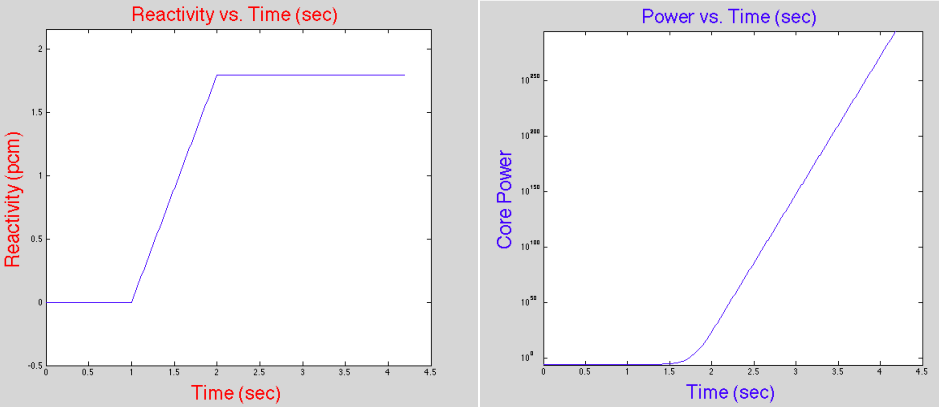
\includegraphics[width=4in]{images/pke/feedback1.png}
    \\
    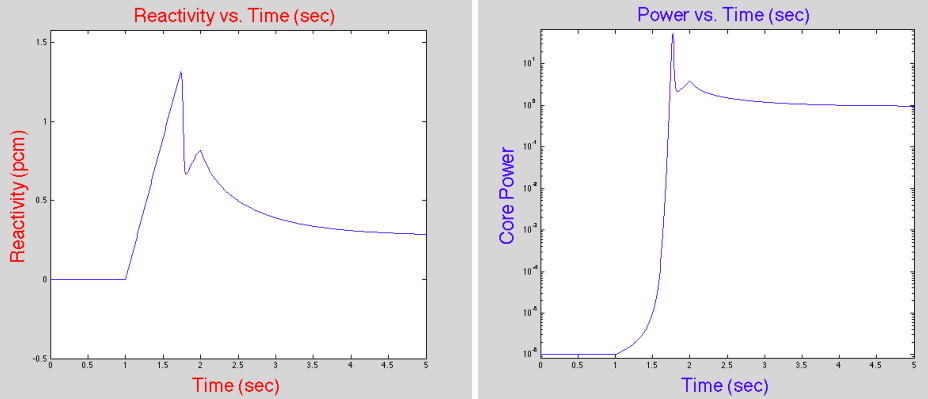
\includegraphics[width=4in]{images/pke/feedback2.png}
    \caption{\$1.5 RIA With or Without Doppler Feedback}\label{feedback}
  \end{figure}



\clearpage
\topic{Fuchs-Nordheim Model}
The Fuchs-Nordheim Model predicts the shape and the magnitude of the transient. We do not really solve the analytical solution of this model, but instead study some characteristics from it. 

\subtopic{Assumptions}
To start, we make three assumptions\footnote{The historical reason for these assumptions is that the model was developed for weapon use, hence $\rho \gg \beta$ and rapid transient.}, 
\begin{enumerate}
\item If $\rho \gg \beta$, we can ignore the delayed neutrons and hence write the power distribution $P(t)$ as the 1st equation in PKE (we use $P(t)$ instead of $T(t)$ for the shape function now to avoid the confusion with temperature $T$ that we would use repeatively in this section). 
  \eqn{ \ddt P(t) &= \frac{\rho(t) - \beta}{\Lambda} P(t) + \Sum_i \lambda_i C_i (t) \approx \frac{\rho(t) - \beta}{\Lambda} P(t) \label{fn-eq1}}
  It is fair to ignore the precursors, because as in Fig.~\ref{fn1} top row, we can see that the power with precursor is small enough that the F-N model provides good approximation. The bottom row of Fig.~\ref{fn1} is plotted on a log-log scale to show the small difference made by the precursors.  
\begin{figure}[ht]
  \centering
  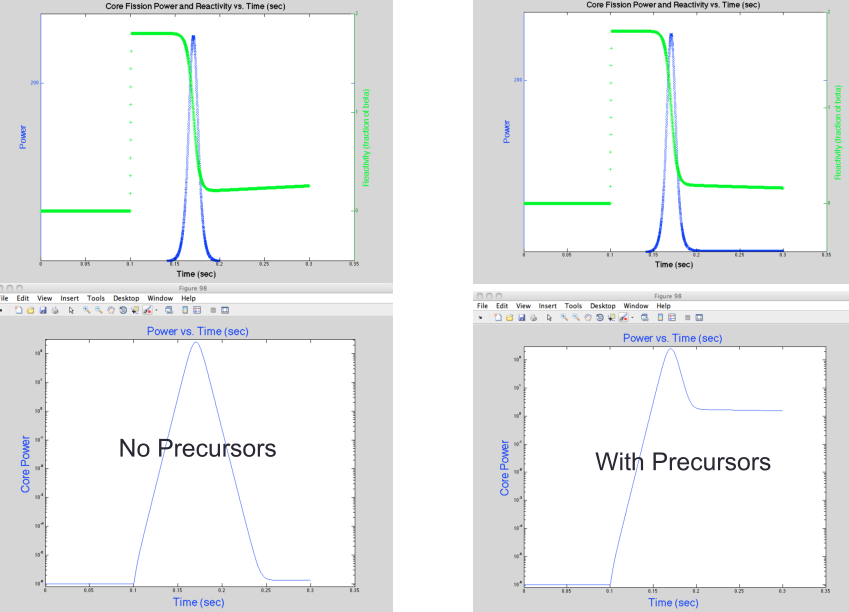
\includegraphics[width=6in]{images/pke/fn1.png}
  \caption{Assumption in Fuchs-Nordheim: No Precursors}\label{fn1}
\end{figure}

\item If transient is so rapid that no heat transferred form the fuel \footnote{The time constant for heat to be removed from \ce{UO_2} fuel is about 5 mins.}, 
  \eqn{ T_{fuel} = T_{fuel}^0 + \frac{1}{C_p} \int P(t) \dt \label{fn-eq2} }

\item Assume a Doppler Feedback coefficient independent of temperature (recall that the doppler we calculated is about 3 pcm), 
  \eqn{ \rho(t) = \rho_{rod} - \alpha (T_{fuel} - T_{fuel}^0) \label{fn-eq3} }
\end{enumerate}

\subtopic{First Derivation}
Then we solve a first order ODE. We differentiate Eq.~\ref{fn-eq2} to get,
\eqn{ \frac{\dT_{fuel} (t)}{\dt} = \frac{P(t)}{C_p} \label{fn-eq4}}
Plug Eq.~\ref{fn-eq3} into Eq.~\ref{fn-eq1} (omit $T_{fuel}^0$), 
\eqn{ \frac{\dP(t)}{\dt} = \frac{\rho_{rod} - \alpha T_{fuel} - \beta}{\Lambda} P(t) \label{fn-eq5} }
Eq.~\ref{fn-eq5} divided by \ref{fn-eq4}, 
\begin{align}
\frac{\dP(t)}{\dT_{fuel}} &= \frac{\frac{\dP(t)}{\dt}}{\frac{\dT_{fuel} (t)}{\dt}} =  \frac{(\rho_{rod} - \alpha T_{fuel} - \beta ) C_p}{\Lambda} \\
&= \frac{1}{\Lambda} \left[ C_p (\rho_{rod} - \beta) - \alpha C_p T_{fuel} (t) \right] \\
\Aboxed{ P(t) &= P_0 + \frac{1}{\Lambda} \left[ C_p (\rho_{rod} - \beta) T_{fuel} (t)  - \frac{\alpha C_p}{2} T^2_{fuel} (t) \right]  } \label{fn-power}
\end{align}
Eq.~\ref{fn-power} can be used to find peak power behavior. For peak power, we set $\frac{\dP}{dT_{fuel}} = 0$, thus, 
\begin{align}
0 &= \frac{1}{\Lambda} \left[ C_p (\rho_{rod} - \beta) - C_p \alpha T_{fuel}^{peak} \right] \\
\Aboxed{ T_{fuel}^{peak} &= \frac{\rho_{rod} - \beta}{\alpha} } \label{fn-11} \\
\Aboxed{ P^{peak} &= P_0 + \frac{C_p (\rho_{rod} - \beta)^2}{2 \Lambda \alpha} }
\end{align}
Take-away: 
\begin{enumerate}
\item \hi{Peak temperature is independent of neutron lifetime and heat capacity.} 
\item Peak power is proportional to $C_p$, and inversely proportional to $\Lambda$. That is, fast reactors with small $\Lambda$ are going to generate a lot of heat in a short amount of time. 
\item Also notice that all of these models are derived with at least $\rho > \beta$. As $\rho \to \beta$, the above equations become very sensitive.
\end{enumerate}


\subtopic{Second Derivation}
Alternatively, we use $\frac{\dP}{\dt}$ expression from the PKEs, and $\frac{\drho}{\dt}$ expression from Eq.~\ref{fn-power} that we derived, 
\begin{align}
\frac{\dP(t)}{\dt} &= \frac{\dP(t)}{\drho} \frac{\drho}{\dt}  \\
\frac{\dP(t)}{\drho} &= \frac{  \frac{\dP(t)}{\dt} }{  \frac{\drho}{\dt} } \\
&= \frac{ \frac{\rho(t) - \beta}{\Lambda} P(t) }{ - \frac{\alpha}{\Lambda C_p } P(t)} \\
&= - \frac{C_p}{\alpha} \left[ \rho(t) - \beta \right] 
\end{align}
We integrate with repsect to $\rho$ and evaluate the constant of integration by using the step reactivity $\rho_{rod}$, 
\eqn{ P(t) = P_0 + \frac{C_p}{2\alpha} \left[ - (\rho(t) - \beta)^2 + (\rho_{rod} - \beta)^2 \right]  }
If we consider the transient terminated when $P(t)$ returns to $P_0$, then 
\eqn{ \rho_{end} = 2 \beta - \rho_{rod} }
Using the constant fuel temperature feedback coefficient, 
\eqn{ 2 \beta - \rho_{rod}  = \rho_{rod} - \alpha (T_{fuel}^{end} - T_{fuel}^0 ) }
That is, 
\eqn{ \Aboxed{ T_{fuel}^{end} &= \frac{2 (\rho_{rod} - \beta)}{\alpha} + T_{fuel}^0 } }
  Compare $T_{fuel}^{end}$ in the above expression with $T_{fuel}^{peak}$ in Eq.~\ref{fn-11}, \textbf{the final temperature is twice the temperature rise at the time of the peak power,} and it is independent of neutron lifetime and heat capacity again. 


\clearpage
\topic{Fuchs-Nordheim Examples}
\begin{enumerate}
\item \hi{Asymptotic fuel temperature is independent of the reactivity insertion rate} as in Fig.~\ref{fn2}. The power vs. time shape changes as we alter reactivity insertion rate. For instance, for 2s, there is a second peak that happens when the rod is fully inserted.  F-N model provides pretty good estimation, because temperature is basically integrated power, and the reactivity insertion rate does not matter that much because we are integrating over time. Another way to think about is that there has to be something to balance out the reactivity change, and it is the Doppler feedback, thus temperature that balance out the reactivity change. Thus the asymptotic temperature only depends on the asymptotic reactivity. 

  \begin{figure}[ht] 
    \centering
    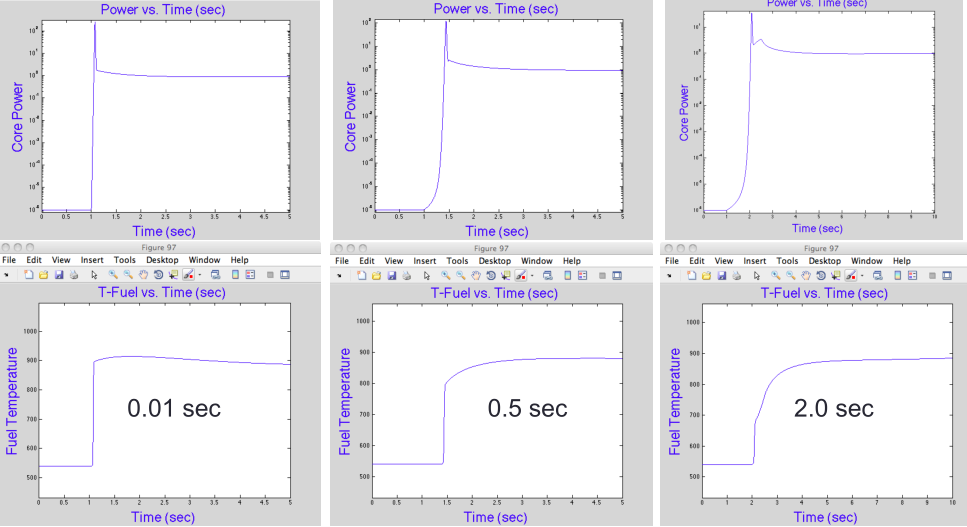
\includegraphics[width=7in]{images/pke/fn2.png}
    \caption{Fuel Temperature Independent Reactivity Insertion Rate} \label{fn2}
  \end{figure}

\item \$1.8 Insertion at Full Power: RIA at full power results in much smaller power increase because we are already at the point of sensible heat addition. Fuel temperature rise is similar to that of RIA from low power. 
  \begin{figure}[ht] 
    \centering
    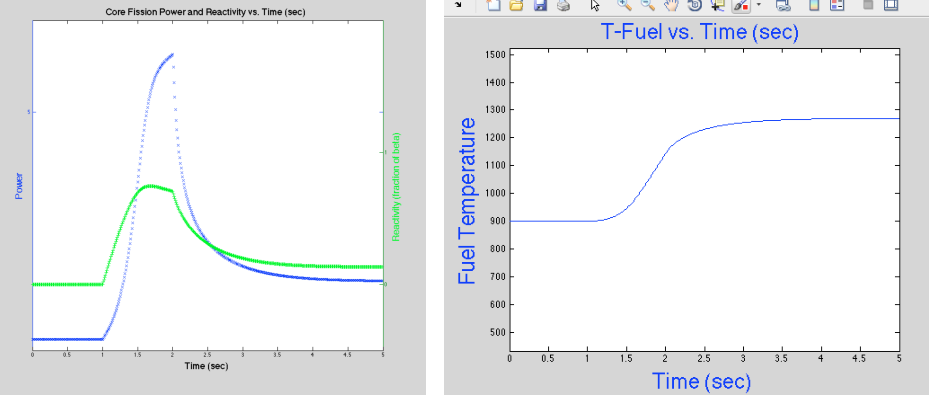
\includegraphics[width=4in]{images/pke/fn3.png}
    \caption{\$1.8 Insertion at Full Power using IK with Feedback}
  \end{figure}

\item As in Fig.~\ref{fn4}, about 3\% of the energy deposited into the coolant (about $2.5 \times 2$ MeV $=$5 MeV worth of neutrons from 200 MeV just from neutron slowing down that is deposited into the coolant), hence the coolant temperature would change slightly as well. Net reactivity comes back to zero.
  \begin{figure}[ht] 
    \centering
    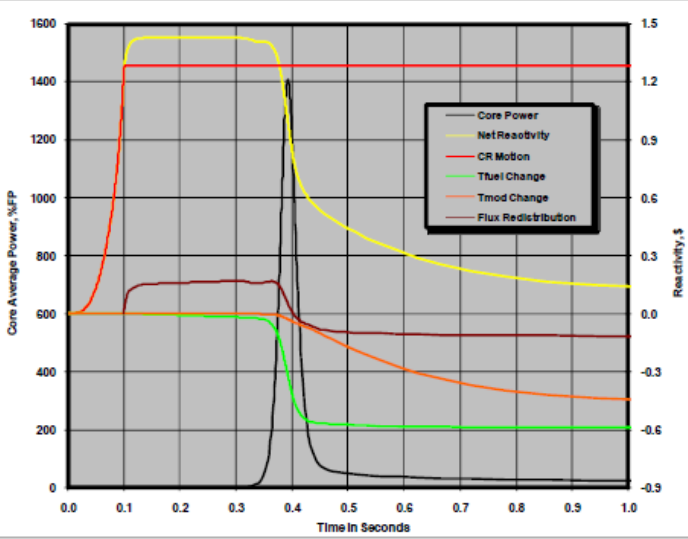
\includegraphics[width=4in]{images/pke/fn4.png}
    \caption{PWR Reactivity Insertion Accident} \label{fn4}
  \end{figure}

\item RIA Safety Analysis: Rod Ejection at HZP. If we have a 1.5\$ RIA without feedback, the power increases very rapidly with an asymptotic period. With Doppler feedback, the feedback is pronound when reactivity is above 1 dollar. A second peak is the characteristic of longer rod change. 
\end{enumerate}

\clearpage
\topic{PKEs with Simple Feedback}
Now we turn away from Fuchs-Nordheim and add some very simple feedbacks into PKEs. We have two first order ODEs, one for $T_{fuel}$, one for $T_{coolant}$. Basically each equation has a source term and a sink term. 
\begin{align}
\ddt T_{fuel} (t) &= a P(t) - b [T_{fuel}(t) - T_{coolant}(t)] \\
\ddt T_{coolant} (t) &= c [T_{fuel}(t) - T_{coolant} (t) ] - d [T_{coolant} (t) - T_{inlet} (t) ] 
\end{align}
Re-write in matrix form, 
\begin{align}
\ddt \left[ \begin{array}{c} T_{fuel}(t) \\ T_{coolant} (t) \end{array} \right]
+ \left[ \begin{array}{cc} b & -b \\ -c & c+d \end{array} \right] 
\left[ \begin{array}{c} T_{fuel} (t) \\ T_{coolant} (t) \end{array} \right] 
= 
\left[ \begin{array}{c} a P_{fuel}(t) \\ d T_{inlet}(t) \end{array} \right]
\end{align}
Using integrating factors to solve the above first order ODE system,  we get, 
\begin{align}
 \left[ \begin{array}{c} T_{fuel}^{n+1} \\ T_{coolant}^{n+1} \end{array} \right]
&= \exp \left\{ -  \left[ \begin{array}{cc} b & -b \\ -c & c+d \end{array} \right] \Delta_t^n \right\}
\left[ \begin{array}{c} T_{fuel}^n \\ T_{coolant}^n \end{array} \right] \\
&+ \exp \left\{ -  \left[ \begin{array}{cc} b & -b \\ -c & c+d \end{array} \right] \Delta_t^n \right\}
\left[ \begin{array}{cc} b & -b \\ -c & c+d \end{array} \right]^{-1}
\exp \left\{ \left[ \begin{array}{cc} b & -b \\ -c & c+d \end{array} \right] \Delta_t^n \right\}
\left[ \begin{array}{c} a P_{fuel}^{n+1} \\ d T_{inlet}^{n+1} \end{array} \right]
\end{align}
We make use of that we know at full power,  flow rate is 30 W/g, $C_p = 300$J/kg-s, $\alpha = -3$ pcm/K, $V_{coolant} = 2 \m/\s, T_{inlet}^0 = 540 \K, T_{coolant}^0 = 560 \K, T_{fuel}^0 = 900 \K$, core height is 4m. 


If power is increasing, we can do TH first and then neutronics. If power is decreasing, 




\clearpage
\topic{Examples of PKEs with Simple Feedbacks}
\begin{enumerate}
\item Ramp reactivity inertion of $0.5\beta$ with feedback. The power decreases because of Doppler feedback and of delayed neutrons. 

\begin{figure}[ht]
  \centering
  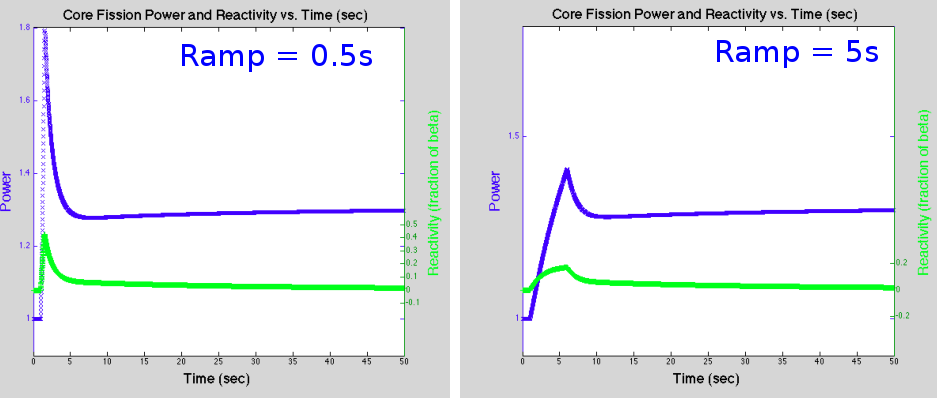
\includegraphics[width=6in]{images/pke/fn5.png}
  \caption{$0.5 \beta$ Reactivity Insertion with Feedback}
\end{figure}

\item Ramp reactivity removal of $0.5\beta$ with feedback. 
\begin{figure}[ht]
  \centering
  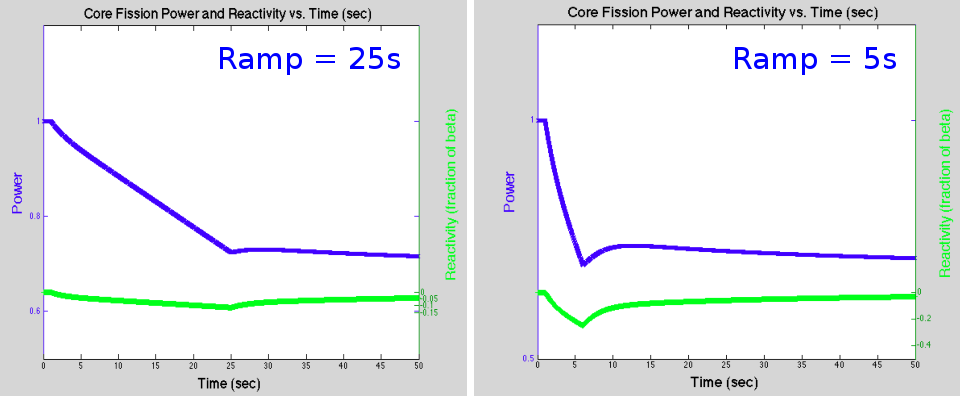
\includegraphics[width=6in]{images/pke/fn6.png}
  \caption{$-0.5 \beta$ Reactivity Insertion with Feedback}
\end{figure}
The slower ramping results in smaller reactivity change (hence smaller peak reactivity for reactivity insertion and larger power dip for negative reactivity insertion), thus smaller power change as well. That is, \textbf{The smaller rate of reactivity change is, the smaller the overshoot is.} But the final/asymptotic results are independent of rate of reactivity insertion, because system always finds stable state. 

Selective ramp insertion: 2 sec, power comes down quickly and recoveries, the radial heat gets high, close to an DNDF failure, makes sure to take into account the power rise. 

Again the asymptotic power level is independent of reactivity changing rate. 


\item 1.5 $\beta$ RIA from HZP with feedback. Power increases by about 100 times. 


\item 1.5 $\beta$ RIA from HFP with feedback. Power increases by about 70 times. Because we start at a higher power region, so we get feedback more quickly this way. The $\Delta T$ is about the same as the HZP because of the reactivity change is the same and our Doppler feedback coefficient is linear. 

\item 1.5 $\beta$ RIA  


\item $1.5 \beta$ bank withdrawal RIA from HFP with feedback: the ejection is so slow that the reactor is at equilibrium the whole time. 
\end{enumerate}
Take-away: we don't really care about the temperal difference/integration, because the asymptotic temperature only depends on the reactivity change, not on the time dependent behavior. 



\clearpage
\topic{Summary}
\begin{enumerate}
\item PKEs assume you are solving for the core average properties; PKEs assume flux spatial shape is constant. Thus PKEs are not very precise for large spatial flux changes. 
\item Peak temperature are proportionally larger than core average properties;
\item If we relly want spatial dynamics, we need to do 3D spatial dynamics to get correct predictions to complicated problems. 
\end{enumerate}
This thermal hydraulics model we have is very crude. For one thing, it has a huge diffusive property, that is, it would not predict any thermal shock behavior. 

\end{document}
